\documentclass[11pt,preprint]{elsarticle}

\usepackage{lmodern}
%%%% My spacing
\usepackage{setspace}
\setstretch{1.2}
\DeclareMathSizes{12}{14}{10}{10}

% Wrap around which gives all figures included the [H] command, or places it "here". This can be tedious to code in Rmarkdown.
\usepackage{float}
\let\origfigure\figure
\let\endorigfigure\endfigure
\renewenvironment{figure}[1][2] {
    \expandafter\origfigure\expandafter[H]
} {
    \endorigfigure
}

\let\origtable\table
\let\endorigtable\endtable
\renewenvironment{table}[1][2] {
    \expandafter\origtable\expandafter[H]
} {
    \endorigtable
}


\usepackage{ifxetex,ifluatex}
\usepackage{fixltx2e} % provides \textsubscript
\ifnum 0\ifxetex 1\fi\ifluatex 1\fi=0 % if pdftex
  \usepackage[T1]{fontenc}
  \usepackage[utf8]{inputenc}
\else % if luatex or xelatex
  \ifxetex
    \usepackage{mathspec}
    \usepackage{xltxtra,xunicode}
  \else
    \usepackage{fontspec}
  \fi
  \defaultfontfeatures{Mapping=tex-text,Scale=MatchLowercase}
  \newcommand{\euro}{€}
\fi

\usepackage{amssymb, amsmath, amsthm, amsfonts}

\def\bibsection{\section*{References}} %%% Make "References" appear before bibliography


\usepackage[numbers]{natbib}

\usepackage{longtable}
\usepackage[margin=2.3cm,bottom=2cm,top=2.5cm, includefoot]{geometry}
\usepackage{fancyhdr}
\usepackage[bottom, hang, flushmargin]{footmisc}
\usepackage{graphicx}
\numberwithin{equation}{section}
\numberwithin{figure}{section}
\numberwithin{table}{section}
\setlength{\parindent}{0cm}
\setlength{\parskip}{1.3ex plus 0.5ex minus 0.3ex}
\usepackage{textcomp}
\renewcommand{\headrulewidth}{0.2pt}
\renewcommand{\footrulewidth}{0.3pt}

\usepackage{array}
\newcolumntype{x}[1]{>{\centering\arraybackslash\hspace{0pt}}p{#1}}

%%%%  Remove the "preprint submitted to" part. Don't worry about this either, it just looks better without it:
\makeatletter
\def\ps@pprintTitle{%
  \let\@oddhead\@empty
  \let\@evenhead\@empty
  \let\@oddfoot\@empty
  \let\@evenfoot\@oddfoot
}
\makeatother

 \def\tightlist{} % This allows for subbullets!

\usepackage{hyperref}
\hypersetup{breaklinks=true,
            bookmarks=true,
            colorlinks=true,
            citecolor=blue,
            urlcolor=blue,
            linkcolor=blue,
            pdfborder={0 0 0}}


% The following packages allow huxtable to work:
\usepackage{siunitx}
\usepackage{multirow}
\usepackage{hhline}
\usepackage{calc}
\usepackage{tabularx}
\usepackage{booktabs}
\usepackage{caption}


\newenvironment{columns}[1][]{}{}

\newenvironment{column}[1]{\begin{minipage}{#1}\ignorespaces}{%
\end{minipage}
\ifhmode\unskip\fi
\aftergroup\useignorespacesandallpars}

\def\useignorespacesandallpars#1\ignorespaces\fi{%
#1\fi\ignorespacesandallpars}

\makeatletter
\def\ignorespacesandallpars{%
  \@ifnextchar\par
    {\expandafter\ignorespacesandallpars\@gobble}%
    {}%
}
\makeatother


% definitions for citeproc citations
\NewDocumentCommand\citeproctext{}{}
\NewDocumentCommand\citeproc{mm}{%
\href{\#cite.\detokenize{#1}}{#2}\nocite{#1}}

\makeatletter
% allow citations to break across lines
\let\@cite@ofmt\@firstofone
% avoid brackets around text for \cite:
\def\@biblabel#1{}
\def\@cite#1#2{{#1\if@tempswa , #2\fi}}
\makeatother
\newlength{\cslhangindent}
\setlength{\cslhangindent}{1.5em}
\newlength{\csllabelwidth}
\setlength{\csllabelwidth}{3em}
\newenvironment{CSLReferences}[2] % #1 hanging-indent, #2 entry-spacing
{\begin{list}{}{%
	\setlength{\itemindent}{0pt}
	\setlength{\leftmargin}{0pt}
	\setlength{\parsep}{0pt}
	% turn on hanging indent if param 1 is 1
	\ifodd #1
	\setlength{\leftmargin}{\cslhangindent}
	\setlength{\itemindent}{-1\cslhangindent}
	\fi
	% set entry spacing
	\setlength{\itemsep}{#2\baselineskip}}}
{\end{list}}

\usepackage{calc}
\newcommand{\CSLBlock}[1]{\hfill\break\parbox[t]{\linewidth}{\strut\ignorespaces#1\strut}}
\newcommand{\CSLLeftMargin}[1]{\parbox[t]{\csllabelwidth}{\strut#1\strut}}
\newcommand{\CSLRightInline}[1]{\parbox[t]{\linewidth - \csllabelwidth}{\strut#1\strut}}
\newcommand{\CSLIndent}[1]{\hspace{\cslhangindent}#1}


\urlstyle{same}  % don't use monospace font for urls
\setlength{\parindent}{0pt}
\setlength{\parskip}{6pt plus 2pt minus 1pt}
\setlength{\emergencystretch}{3em}  % prevent overfull lines
\setcounter{secnumdepth}{5}

%%% Use protect on footnotes to avoid problems with footnotes in titles
\let\rmarkdownfootnote\footnote%
\def\footnote{\protect\rmarkdownfootnote}
\IfFileExists{upquote.sty}{\usepackage{upquote}}{}

%%% Include extra packages specified by user

%%% Hard setting column skips for reports - this ensures greater consistency and control over the length settings in the document.
%% page layout
%% paragraphs
\setlength{\baselineskip}{12pt plus 0pt minus 0pt}
\setlength{\parskip}{12pt plus 0pt minus 0pt}
\setlength{\parindent}{0pt plus 0pt minus 0pt}
%% floats
\setlength{\floatsep}{12pt plus 0 pt minus 0pt}
\setlength{\textfloatsep}{20pt plus 0pt minus 0pt}
\setlength{\intextsep}{14pt plus 0pt minus 0pt}
\setlength{\dbltextfloatsep}{20pt plus 0pt minus 0pt}
\setlength{\dblfloatsep}{14pt plus 0pt minus 0pt}
%% maths
\setlength{\abovedisplayskip}{12pt plus 0pt minus 0pt}
\setlength{\belowdisplayskip}{12pt plus 0pt minus 0pt}
%% lists
\setlength{\topsep}{10pt plus 0pt minus 0pt}
\setlength{\partopsep}{3pt plus 0pt minus 0pt}
\setlength{\itemsep}{5pt plus 0pt minus 0pt}
\setlength{\labelsep}{8mm plus 0mm minus 0mm}
\setlength{\parsep}{\the\parskip}
\setlength{\listparindent}{\the\parindent}
%% verbatim
\setlength{\fboxsep}{5pt plus 0pt minus 0pt}



\begin{document}



\begin{frontmatter}  %

\title{Question 1}

% Set to FALSE if wanting to remove title (for submission)




\author[Add1]{Vincent Reinshagen}
\ead{\href{mailto:28736907@sun.ac.za}{\nolinkurl{28736907@sun.ac.za}}}





\address[Add1]{Stellenbosch University}



\vspace{1cm}





\vspace{0.5cm}

\end{frontmatter}

\setcounter{footnote}{0}



%________________________
% Header and Footers
%%%%%%%%%%%%%%%%%%%%%%%%%%%%%%%%%
\pagestyle{fancy}
\chead{}
\rhead{}
\lfoot{}
\rfoot{}
\lhead{}
%\rfoot{\footnotesize Page \thepage } % "e.g. Page 2"
\cfoot{}

%\setlength\headheight{30pt}
%%%%%%%%%%%%%%%%%%%%%%%%%%%%%%%%%
%________________________

\headsep 35pt % So that header does not go over title




I will start my analysis using the PerfomanceAnalytics package, to make
use of this package, it is necessary to spread the data. Since we also
want to compare the AI Fund to managed funds, I created the function
mean\_A which calculates the returns across all funds for each date. The
format of the three datasets now allows to merge them. Furthermore, the
columns are renamed for clarity. The merged dataset can then be used to
plot a cumulative return chart.

The plot shows, that the AI Fund (black line) shows a notably higher
cumulative return compared to the Benchmark (green line) and Managed
Funds (red line). The Managed Funds perform consistently below both the
Benchmark and AI Fund over time.

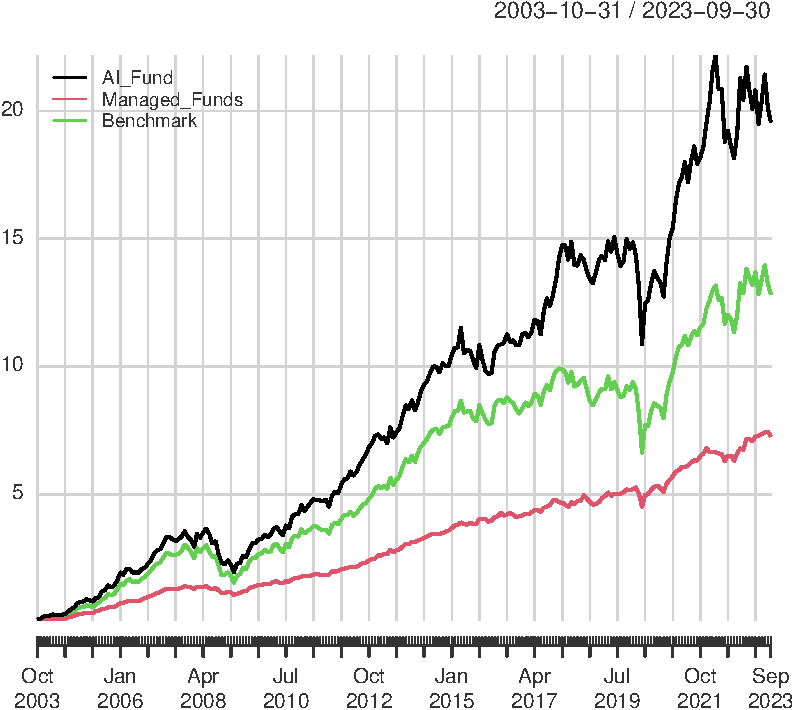
\includegraphics{Question1_files/figure-latex/unnamed-chunk-3-1.pdf}

After calculating cumulative returns to assess overall performance,
rolling returns are analyzed to evaluate consistency and resilience over
different time periods, addressing potential biases from early outcomes
or isolated events.

This plot aligns with the general conclusions from the previous plot but
provides a more granular view of short-term performance trends over
time.

While the previous chart highlighted the AI Fund's superior cumulative
returns, this chart shows that the AI Fund's rolling 12-month returns
are more volatile but still consistently outperform the Benchmark and
Managed Funds over longer periods. The AI Fund exhibits higher peaks and
lower troughs compared to the others, suggesting higher risk but also
higher reward. Managed Funds consistently exhibit lower volatility and
returns, staying below the AI Fund and often below the Benchmark.

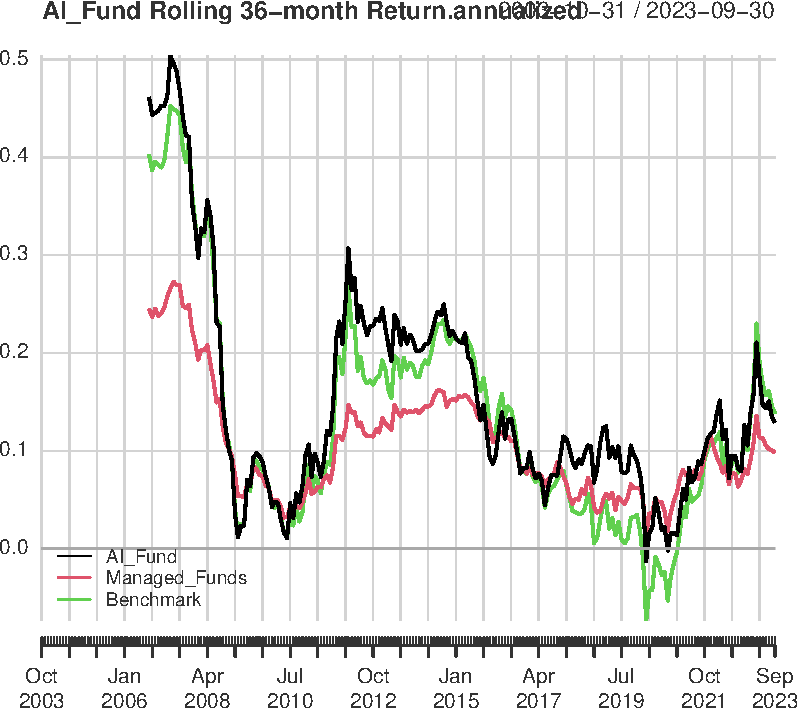
\includegraphics{Question1_files/figure-latex/unnamed-chunk-4-1.pdf}

This density plot complements the earlier findings: The AI Fund (red)
has a broader and flatter distribution, indicating higher variance and a
wider range of returns. Its mean is higher than both the Benchmark and
Managed Funds, reinforcing its superior performance over time. The
Managed Funds (blue) show a narrower distribution, reflecting lower
variability in returns. However, its mean is the lowest among the three
datasets, confirming its consistent underperformance relative to the AI
Fund and the Benchmark.The Benchmark (green) displays a middle ground,
with a tighter distribution compared to the AI Fund but slightly wider
than the Managed Funds. Its mean return is higher than Managed Funds but
below the AI Fund.

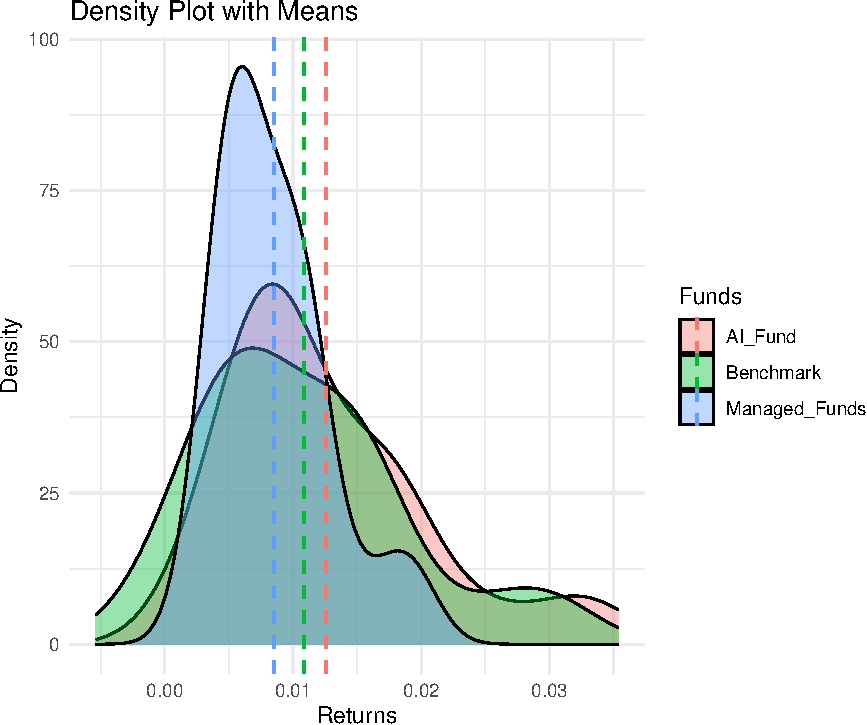
\includegraphics{Question1_files/figure-latex/unnamed-chunk-5-1.pdf}

The density plot with variances confirms that the AI Fund, while
offering higher returns, also comes with increased risk compared to the
other two datasets. Managed Funds provide the most stability but
underperform in terms of both returns and risk-adjusted performance.

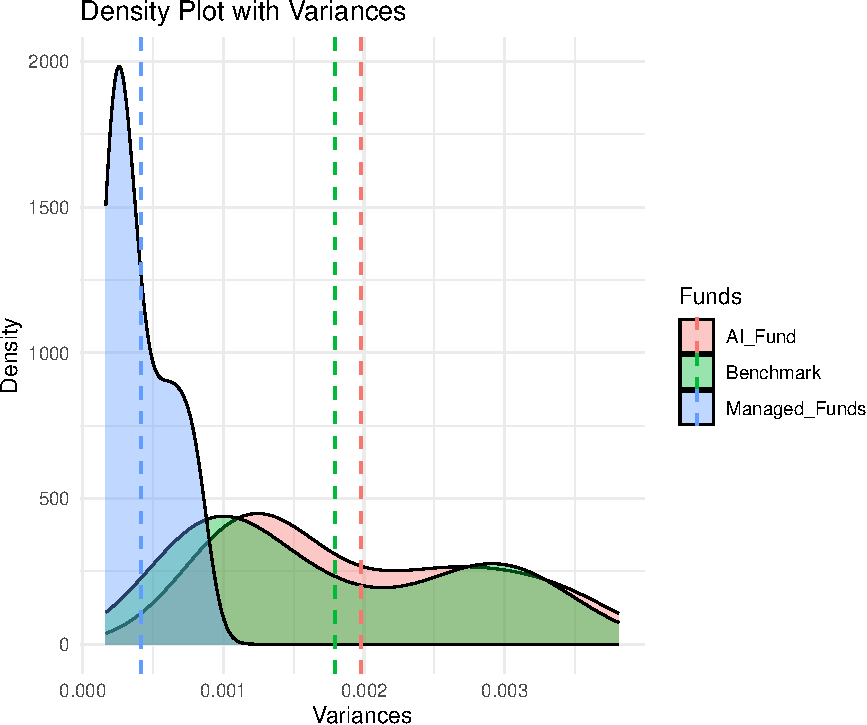
\includegraphics{Question1_files/figure-latex/unnamed-chunk-6-1.pdf}

Rolling plot already shows lowest variance for Managed funds, and
highest variance for AI fund The drawdown chart emphasizes the AI Fund's
greater susceptibility to sharp declines, despite its long-term
outperformance.

\begin{verbatim}
##                                 AI_Fund Managed_Funds  Benchmark
## Downside Deviation (MAR = 0%) 0.0258682    0.01085863 0.02497928
\end{verbatim}

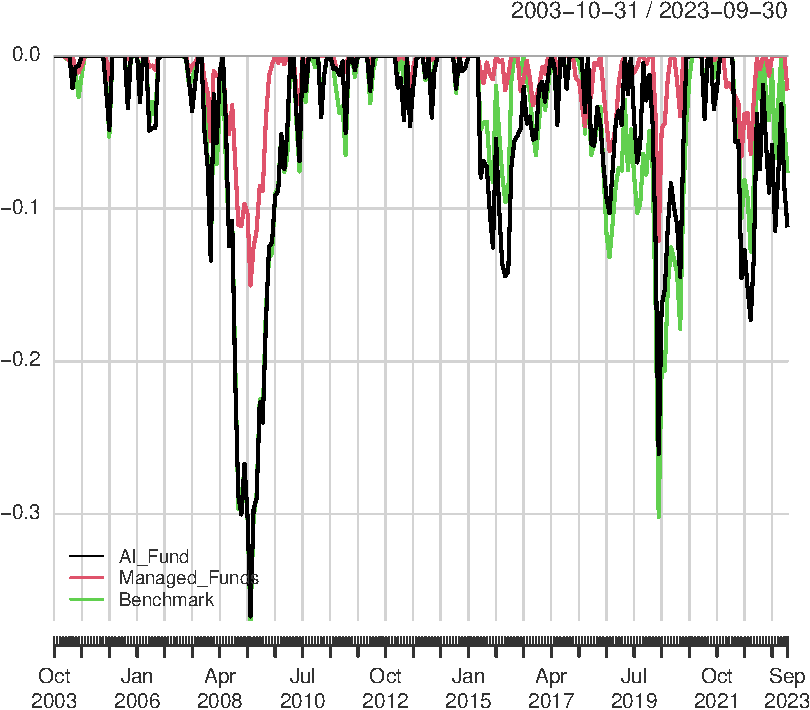
\includegraphics{Question1_files/figure-latex/unnamed-chunk-7-1.pdf}

The analysis highlights that the AI Fund consistently outperforms both
the Benchmark and Managed Funds in terms of returns, albeit with higher
volatility and deeper drawdowns. While Managed Funds offer lower risk
and more stability, they underperform in both mean and cumulative
returns. The Benchmark provides a moderate balance of risk and
performance but cannot match the AI Fund's long-term growth. This
suggests the AI Fund is better suited for risk-tolerant investors
seeking higher returns, while Managed Funds cater to more conservative
strategies.

\bibliography{Tex/ref}





\end{document}
